\documentclass{ieeetj}
\usepackage{cite}
\usepackage{amsmath,amssymb,amsfonts}
\usepackage{listings}
\usepackage{algorithmic}
\usepackage{graphicx,color}
\usepackage{textcomp}
\usepackage{xcolor}
\usepackage{hyperref}
\hypersetup{hidelinks=true}
\usepackage{algorithm,algorithmic}
\def\BibTeX{{\rm B\kern-.05em{\sc i\kern-.025em b}\kern-.08em
    T\kern-.1667em\lower.7ex\hbox{E}\kern-.125emX}}
\AtBeginDocument{\definecolor{tmlcncolor}{cmyk}{0.93,0.59,0.15,0.02}\definecolor{NavyBlue}{RGB}{0,86,125}}

% Definim el logo
\def\OJlogo{
    \vspace{-14pt} % Espai negatiu per pujar el logo
    
\includegraphics[height=0.96cm]{png/logo.png}}

\begin{document}
\receiveddate{20 Febrer, 2025}
\publisheddate{12 Març, 2025}
\currentdate{12 Març, 2025}

\title{Implementació del Model Vista Controlador en una Aplicació Pràctica}

\author{Josep Ferriol, Daniel García, Khaoula Ikkene, Biel Perelló}
\affil{Universitat de les Illes Balears, Departament d'Enginyeria Informàtica}
\corresp{Autor de contacte: Daniel García (email: daniel.garcia19@estudiant.uib.es)}

\begin{abstract}
Aquest document presenta la implementació del Model Vista Controlador (MVC) en una aplicació pràctica. Es detallen els conceptes teòrics de l’arquitectura MVC, el patró per esdeveniments i el càlcul del cost asimptòtic de la instrucció crítica. A més, es descriu l'entorn de programació utilitzat, incloent les llibreries de Swing per a la interfície gràfica. La pràctica consisteix en desenvolupar una aplicació que implementi els algorismes de suma i producte de matrius. Es presenten gràfiques dels costos computacionals assimptòtics d'aquests algorismes, així com una anàlisi del temps d'execució i la constant multiplicativa. L'aplicació permet iniciar i arrancar els processos de suma i producte de matrius i mostra els resultats en una interfície gràfica desenvolupada amb Java Swing.

Finalment, s'analitzen els resultats obtinguts i es presenten les conclusions del projecte.
\end{abstract}

\begin{IEEEkeywords}
Arquitectura de Programari, Cost Asimptòtic, Java Swing, Model-Vista-Controlador, Multiplicació de Matrius, Programació Basada en Esdeveniments, Suma de Matrius
\end{IEEEkeywords}

\maketitle
\section{Introducció}
El Model Vista Controlador (MVC) és un patró d'arquitectura de programari àmpliament utilitzat per separar la lògica de presentació, la lògica de negoci i la gestió de dades. Aquesta separació permet millorar la modularitat i mantenibilitat dels sistemes, facilitant així el desenvolupament i manteniment de les aplicacions.

Aquest projecte té com a objectiu implementar el patró MVC en una aplicació pràctica que realitzi operacions de suma i producte de matrius. A més, es pretén analitzar els beneficis d'aquest patró en termes de modularitat i eficiència.

En aquesta memòria, es presenten els conceptes teòrics de l'arquitectura MVC, incloent la seva estructura i els avantatges que ofereix. També s'explica el patró per esdeveniments, que permet una comunicació eficient entre els components del sistema mitjançant la gestió d'esdeveniments i notificacions.

A continuació, es descriu l'entorn de programació utilitzat per al desenvolupament de l'aplicació, incloent les llibreries de Swing per a la interfície gràfica i les eines emprades per a la gestió del codi i el control de versions.

La part central de la pràctica consisteix en desenvolupar una aplicació que implementi els algorismes de suma i producte de matrius, amb complexitats O(n\textsuperscript{2}) i O(n\textsuperscript{3}) respectivament. Es presenten gràfiques dels costos computacionals asimptòtics d'aquests algorismes, així com una anàlisi detallada del temps d'execució i la constant multiplicativa. L'aplicació permet iniciar i arrancar els processos de suma i producte de matrius, junts o per separat, i mostra els resultats en una interfície gràfica desenvolupada amb Java Swing.

Finalment, s'analitzen els resultats obtinguts, destacant els beneficis de l'ús del patró MVC en termes de modularitat i mantenibilitat del codi. També es presenten les conclusions del projecte i es proposen possibles millores futures per optimitzar el sistema.

\section{Conceptes Teòrics}
\subsection{Model Vista Controlador (MVC)}
El Model Vista Controlador (MVC) és un patró d'arquitectura de programari que separa l'aplicació en tres components principals: el Model, la Vista i el Controlador. Aquesta separació permet una millor modularitat i mantenibilitat del codi.

\begin{itemize}
    \item \textbf{Model}: Gestiona les dades i la lògica de negoci de l'aplicació. És responsable de l'accés a la base de dades, càlculs i qualsevol altra lògica de negoci necessària. La lògica de negoci, també coneguda com a lògica de l'aplicació, és un conjunt de regles que es segueixen en el programari per reaccionar davant diferents situacions. A més de marcar un comportament quan ocorren coses dins del programari, també té normes sobre el que es pot fer i el que no es pot fer, conegudes com a regles del negoci.
    \item \textbf{Vista}: S'encarrega de la presentació de les dades a l'usuari. És responsable de la interfície gràfica i de mostrar la informació de manera comprensible. La Vista actua com el frontend o interfície gràfica d'usuari (GUI).
    \item \textbf{Controlador}: Actua com a intermediari entre el Model i la Vista. Gestiona les interaccions de l'usuari, actualitza el Model i refresca la Vista. El Controlador és el cervell de l'aplicació que controla com es mostren les dades.
\end{itemize}

\begin{figure}[htbp]
\centerline{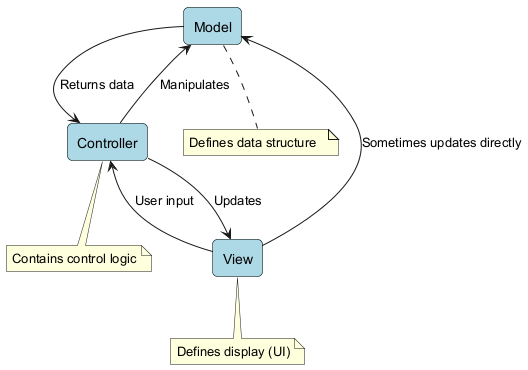
\includegraphics[width=0.45\textwidth]{png/MVC.png}}
\caption{Esquema del Model-Vista-Controlador.}
\label{fig:mvc}
\end{figure}

El concepte de MVC va ser introduït per primera vegada per \href{https://en.wikipedia.org/wiki/Trygve_Reenskaug}{Trygve Reenskaug}
, qui el va proposar com una forma de desenvolupar el GUI d'aplicacions d'escriptori. Avui en dia, el patró MVC s'utilitza per a aplicacions web modernes perquè permet que l'aplicació sigui escalable, mantenible i fàcil d'expandir.

Les principals utilitats del patró MVC inclouen:
\begin{itemize}
    \item \textbf{Modularitat}: Facilita la separació de responsabilitats, permetent que cada component es desenvolupi i es mantingui de manera independent. Això respecta el principi de la responsabilitat única, on una part del codi no ha de saber què fa tota l'aplicació, només ha de tenir una responsabilitat específica.
    \item \textbf{Reutilització de codi}: Els components poden ser reutilitzats en diferents parts de l'aplicació o en altres projectes.
    \item \textbf{Facilitat de manteniment}: La separació de responsabilitats facilita la detecció i correcció d'errors, així com la implementació de noves funcionalitats.
    \item \textbf{Separació de preocupacions (SoC)}: El patró MVC ajuda a dividir el codi frontend i backend en components separats, fent que sigui molt més fàcil gestionar i fer canvis a qualsevol dels costats sense que interfereixin entre si.
\end{itemize}

El patró MVC és especialment útil quan diversos desenvolupadors necessiten actualitzar, modificar o depurar una aplicació completada simultàniament. Aquesta separació de preocupacions permet que els desenvolupadors treballin en diferents parts de l'aplicació sense afectar altres parts del codi.

En resum, el patró MVC és una eina poderosa per a la construcció d'aplicacions escalables i mantenibles, permetent una clara separació de responsabilitats i facilitant la gestió del codi.

\subsection{Patró per Esdeveniments}
El patró per esdeveniments és un mecanisme de comunicació entre components que permet gestionar esdeveniments i notificacions de manera eficient. En aquest patró, els components poden generar esdeveniments i subscriure's a esdeveniments generats per altres components.

\begin{itemize}
    \item \textbf{Generació d'esdeveniments}: Els components poden generar esdeveniments quan es produeixen canvis en el seu estat o quan es completen determinades accions.
    \item \textbf{Subscripció a esdeveniments}: Els components poden subscriure's a esdeveniments generats per altres components per rebre notificacions i actuar en conseqüència.
    \item \textbf{Desacoblament}: El patró per esdeveniments permet desacoblar els components, ja que no necessiten conèixer els detalls dels altres components amb els quals interactuen.
\end{itemize}

\subsection{Càlcul del Cost Asimptòtic}
El càlcul del cost asimptòtic és una tècnica utilitzada per analitzar l'eficiència dels algorismes en termes de temps d'execució i ús de memòria. Es basa en la notació Big-O, que descriu el comportament asimptòtic d'un algorisme quan la mida de les dades d'entrada tendeix a l'infinit.

La notació Big-O és una forma de mesurar com escala un programa o un algorisme i el temps que tardarà a executar-se. Aquesta mesura és útil per comparar l'eficiència de dos algorismes, per exemple, d'ordenació. Big-O no proporciona una mesura exacta del temps d'execució, sinó una avaluació de com de ràpid s'incrementa el temps d'execució en funció de les dades d'entrada. En termes matemàtics, descriu el límit d'una funció quan els arguments d'entrada tendeixen a l'infinit o a un valor en particular.

\begin{itemize}
    \item \textbf{Notació Big-O}: Descriu el pitjor cas del temps d'execució d'un algorisme en funció de la mida de les dades d'entrada. Per exemple, O(n\textsuperscript{2}) indica que el temps d'execució creix quadràticament amb la mida de les dades.
    \item \textbf{Cost asimptòtic de la instrucció crítica}: En aquest projecte, s'analitza el cost asimptòtic de les operacions de suma i producte de matrius, amb complexitats O(n\textsuperscript{2}) i O(n\textsuperscript{3}) respectivament.
\end{itemize}

Els diferents tipus de temps de Big-O inclouen:
\begin{itemize}
    \item \textbf{Temps Constant O(1)}: El temps d'execució es manté constant independentment de la mida del conjunt de dades d'entrada.
    \item \textbf{Temps Logarítmic O(log n)}: El temps d'execució depèn del logaritme de la mida del conjunt de dades d'entrada. Per exemple, els algorismes que divideixen el conjunt de dades d'entrada en meitats segueixen aquesta notació.
    \item \textbf{Temps Lineal O(n)}: El temps d'execució depèn directament de la mida del conjunt de dades d'entrada. Com més elements s'afegeixin al processament, el temps d'execució s'incrementarà proporcionalment.
    \item \textbf{Temps Quadràtic O(n\textsuperscript{2})}: El creixement del temps d'execució és exponencial, generalment observat en funcions amb bucles anidats.
    \item \textbf{Temps Exponencial O(2\textsuperscript{n})}: El temps d'execució es duplica amb cada element que s'afegeix al conjunt de dades d'entrada.
    \item \textbf{Temps Factorial O(n!)}: El creixement del temps d'execució és pràcticament vertical, incrementant considerablement amb cada element afegit al conjunt de dades d'entrada.
\end{itemize}

\begin{figure}[htbp]
\centerline{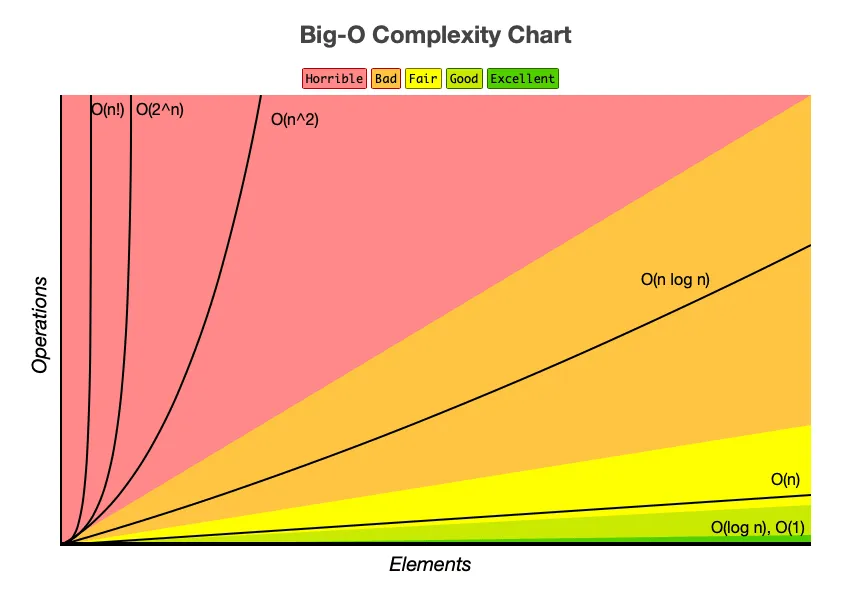
\includegraphics[width=0.45\textwidth]{png/bigO.png}}
\caption{Exemple de diferents complexitats de la notació Big-O.}
\label{fig:big_o}
\end{figure}

La notació Big-O és important perquè permet als desenvolupadors i científics de dades avaluar i comparar l'eficiència de diferents algorismes. Això ajuda a triar l'algorisme més adequat per a una tasca específica, optimitzant el rendiment d'aplicacions i sistemes.

Per calcular la notació Big-O d'un algorisme, s'analitzen els bucles, bucles anidats, recursions i operacions dominants del codi, que són les que més afecten el temps d'execució. A més, un factor important que afecta el rendiment i l'eficiència del programa és el maquinari, el sistema operatiu i la CPU que s'utilitza. No obstant això, això no es té en compte quan s'analitza el rendiment d'un algorisme. En canvi, el que importa és la complexitat temporal i espacial en funció de la mida de l'entrada.

En resum, la notació Big-O és una eina essencial per avaluar l'eficiència dels algorismes i triar els més adequats per a cada situació, optimitzant així el rendiment de les aplicacions.

\subsection{Conceptes Bàsics}
En aquest apartat es presenten alguns conceptes fonamentals que són rellevants per a la implementació del patró MVC i l'anàlisi dels algorismes utilitzats en la pràctica.

El llenguatge de programació és un factor important que pot influir en l'eficiència i la facilitat de desenvolupament d'una aplicació. En aquest projecte, s'ha utilitzat Java, un llenguatge orientat a objectes que facilita la modularitat i la reutilització del codi.

La Programació Orientada a Objectes (POO) és una metodologia de programació que organitza el codi en classes i objectes, permetent una millor estructuració i mantenibilitat del sistema. Les interfícies, per la seva banda, defineixen un contracte que les classes han d'implementar, facilitant la interoperabilitat entre diferents components del sistema.

La separació de la visió, el control i les dades és un principi fonamental del patró MVC. Aquesta separació permet que cada component es desenvolupi i es mantingui de manera independent, millorant la modularitat i la mantenibilitat del sistema.

L'eficiència dels algorismes és un aspecte crucial per al rendiment del sistema. En aquest projecte, s'han implementat algorismes de suma i producte de matrius amb complexitats O(n\textsuperscript{2}) i O(n\textsuperscript{3}) respectivament. La notació Big-O permet descriure el comportament asimptòtic d'aquests algorismes quan la mida de les dades d'entrada tendeix a l'infinit.

És important tenir en compte les mides asimptòtiques i les regles pràctiques per fer primeres aproximacions sobre l'eficiència dels algorismes. Tot i que alguns algorismes poden tenir una bondat teòrica, és important considerar les constants multiplicatives i la balança entre l'eficiència i el cost de producció, així com entre la memòria i el temps d'execució.

Aquests conceptes bàsics proporcionen una base sòlida per a la implementació del patró MVC i l'anàlisi dels algorismes utilitzats en aquest projecte.

\section{Entorn de Programació}
Per al desenvolupament d'aquest projecte s'ha emprat un conjunt d'eines i tecnologies que han facilitat la implementació del patró MVC i l'anàlisi dels algorismes de suma i producte de matrius. A continuació, es descriuen les principals eines utilitzades:

\begin{itemize}
    \item \textbf{Llenguatge de programació: Java} \\
    Java és un llenguatge de programació orientat a objectes que ofereix una gran portabilitat i una àmplia gamma de llibreries i eines per al desenvolupament d'aplicacions. La seva sintaxi clara i la seva robustesa el fan ideal per a projectes que requereixen una alta mantenibilitat i escalabilitat. A més, Java és independent de la plataforma, la qual cosa permet executar l'aplicació en diferents sistemes operatius sense necessitat de modificar el codi.

    \item \textbf{Llibreries utilitzades: Swing} \\
    Swing és una llibreria de Java per a la creació d'interfícies gràfiques d'usuari (GUI). Proporciona un conjunt complet de components gràfics, com ara botons, camps de text, taules i panells, que permeten construir interfícies d'usuari riques i interactives. Swing és altament personalitzable i permet crear interfícies gràfiques que s'adapten a les necessitats específiques de l'aplicació.

    \item \textbf{IDE: IntelliJ IDEA} \\
    IntelliJ IDEA és un entorn de desenvolupament integrat (IDE) per a Java que ofereix una àmplia gamma de funcionalitats per a facilitar el desenvolupament d'aplicacions. Algunes de les seves característiques més destacades inclouen la completació de codi intel·ligent, la navegació ràpida pel codi, les eines de refactorització i la integració amb sistemes de control de versions. Aquestes funcionalitats ajuden a millorar la productivitat i a mantenir un codi net i organitzat.

    \item \textbf{Control de versions: GitHub} \\
    GitHub és una plataforma de desenvolupament col·laboratiu que utilitza el sistema de control de versions Git. Permet gestionar el codi font del projecte, fer seguiment dels canvis, col·laborar amb altres membres de l'equip i mantenir un historial complet de les modificacions realitzades. GitHub també ofereix eines per a la gestió de projectes, com ara issues i pull requests, que faciliten la coordinació i la revisió del codi.
\end{itemize}

L'ús d'aquestes eines i tecnologies ha permès desenvolupar una aplicació robusta i mantenible, seguint els principis del patró MVC i assegurant una bona gestió del codi i la col·laboració entre els membres de l'equip.

\section{Desenvolupament}
En aquesta secció es descriu el desenvolupament de la pràctica, que consisteix en la implementació d'una aplicació basada en el patró Model Vista Controlador (MVC) i el patró per esdeveniments. L'aplicació permet realitzar operacions de suma i producte de matrius, mostrant els costos computacionals asimptòtics d'aquests algorismes.

\subsection{Arquitectura MVC}
L'aplicació està estructurada seguint el patró MVC, que separa la lògica de negoci, la interfície d'usuari i el control de la interacció en tres components principals:

\begin{itemize}
    \item \textbf{Model}: La classe \texttt{Dades} gestiona les dades de l'aplicació, incloent els resultats de les operacions de suma i producte de matrius. Aquesta classe també calcula les constants multiplicatives i emmagatzema els resultats en llistes. La classe \texttt{Matriu} representa una matriu i proporciona mètodes per sumar i multiplicar matrius.
    \item \textbf{Vista}: Les classes \texttt{FinestraMatriu}, \texttt{dibuixConstantMult} i \texttt{Eixos} s'encarreguen de la presentació de les dades a l'usuari. Utilitzen la llibreria Swing per crear la interfície gràfica i mostrar els resultats de les operacions en taules i gràfics.
    \item \textbf{Controlador}: La classe \texttt{Main} actua com a controlador, gestionant les interaccions de l'usuari i coordinant les operacions entre el model i la vista. Aquesta classe és responsable de crear i gestionar els fils d'execució per a les operacions de suma i producte de matrius, així com de mantenir la comunicació entre els diferents components de l'aplicació.

La classe \texttt{Main} conté els següents elements principals:

\begin{itemize}
    \item \textbf{Inicialització}: El mètode \texttt{main} és el punt d'entrada de l'aplicació. Aquest mètode crea una instància de la classe \texttt{Main} i crida al mètode \texttt{inicio} per iniciar l'aplicació. El mètode \texttt{inicio} inicialitza les dades, els processos i l'\texttt{ExecutorService}, i després crida al mètode \texttt{crearInterficie} per crear la interfície gràfica en un fil separat.
    
    \item \textbf{Creació de la Interfície Gràfica}: El mètode \texttt{crearInterficie} crea la finestra principal de l'aplicació utilitzant la classe \texttt{FinestraMatriu}. També crea una segona finestra per mostrar els resultats de les operacions de suma i producte de matrius utilitzant la classe \texttt{dibuixConstantMult}. Aquestes finestres es mostren a l'usuari i permeten la interacció amb l'aplicació.
    
    \item \textbf{Gestió de Processos}: El mètode \texttt{preparar} s'encarrega de buidar les dades i aturar qualsevol procés en execució abans de començar una nova operació. Això assegura que les dades anteriors no interfereixin amb les noves operacions.
    
    \item \textbf{Comunicació}: La classe \texttt{Main} implementa la interfície \texttt{Comunicar}, que defineix el mètode \texttt{comunicar}. Aquest mètode s'utilitza per rebre missatges de la interfície gràfica i dels fils d'execució, i per enviar missatges als components corresponents. Per exemple, quan l'usuari fa clic en un botó per iniciar una operació, es crida al mètode \texttt{comunicar} amb el missatge corresponent, que després es processa per iniciar els fils d'execució adequats.
    
    \item \textbf{Gestió de Fils d'Execució}: La classe \texttt{Main} utilitza un \texttt{ExecutorService} per gestionar els fils d'execució de les operacions de suma i producte de matrius. Quan es rep un missatge per iniciar una operació, es creen instàncies de les classes \texttt{SumaM} i \texttt{MultM} i s'envien al \texttt{ExecutorService} per ser executades en fils separats. Això permet executar les operacions de manera concurrent i millorar l'eficiència de l'aplicació.
    
    \item \textbf{Actualització de la Interfície Gràfica}: Quan es completen les operacions de suma i producte de matrius, els resultats es mostren a la interfície gràfica. La classe \texttt{Main} s'encarrega d'enviar missatges a les classes \texttt{FinestraMatriu} i \texttt{dibuixConstantMult} per actualitzar les taules i els gràfics amb els nous resultats. Això permet a l'usuari visualitzar els costos computacionals asimptòtics de les operacions.
\end{itemize}

En resum, la classe \texttt{Main} actua com a controlador central de l'aplicació, gestionant les interaccions de l'usuari, coordinant les operacions entre el model i la vista, i assegurant que les operacions es realitzin de manera eficient i concurrent. Aquesta arquitectura permet una clara separació de responsabilitats, millorant la modularitat i mantenibilitat del codi.
\end{itemize}

\subsection{Implementació del Patró per Esdeveniments}
L'aplicació utilitza el patró per esdeveniments per gestionar la comunicació entre els components de manera eficient. Aquest patró permet que els components es comuniquin entre ells mitjançant l'enviament i la recepció de missatges, sense necessitat de conèixer els detalls interns dels altres components.

\subsubsection{Interfície \texttt{Comunicar}}
La interfície \texttt{Comunicar} defineix un mètode \texttt{comunicar} que permet enviar missatges entre els components. Aquesta interfície és implementada per diverses classes de l'aplicació, permetent una comunicació uniforme i consistent. La definició de la interfície és la següent:

\begin{lstlisting}[language=Java, basicstyle=\ttfamily\normalsize]
public interface Comunicar {
    public void comunicar(String s);
}
\end{lstlisting}

\subsubsection{Classe \texttt{Main}}
La classe \texttt{Main} actua com a controlador central de l'aplicació i és responsable de gestionar la comunicació entre els components, com s'ha explicat anteriorment. Quan l'usuari interactua amb la interfície gràfica, la classe \texttt{Main} rep els missatges corresponents i els processa per iniciar, aturar o actualitzar les operacions de suma i producte de matrius. El mètode \texttt{comunicar} de la classe \texttt{Main} processa els missatges i crida als mètodes adequats per gestionar les operacions.

\subsubsection{Classes \texttt{SumaM} i \texttt{MultM}}
Les classes \texttt{SumaM} i \texttt{MultM} implementen la interfície \texttt{Comunicar} per rebre missatges del controlador i aturar els fils d'execució quan sigui necessari. Quan es rep un missatge per aturar l'operació, el mètode \texttt{comunicar} d'aquestes classes estableix una variable booleana \texttt{stop} a \texttt{true}, la qual cosa fa que el bucle principal del mètode \texttt{run} s'aturi.

\subsubsection{Classe \texttt{FinestraMatriu}}
La classe \texttt{FinestraMatriu} també implementa la interfície \texttt{Comunicar} per rebre missatges del controlador i actualitzar la interfície gràfica en conseqüència. Per exemple, quan es rep un missatge per iniciar una operació, la classe \texttt{FinestraMatriu} activa les barres de progrés corresponents per indicar que l'operació està en marxa. Quan es rep un missatge per aturar l'operació, les barres de progrés es desactiven.

\subsubsection{Flux de Comunicació}
El flux de comunicació entre els components es pot resumir en els següents passos:

\begin{enumerate}
    \item L'usuari interactua amb la interfície gràfica, per exemple, fent clic en un botó per iniciar una operació.
    \item La classe \texttt{FinestraMatriu} envia un missatge al controlador (classe \texttt{Main}) mitjançant el mètode \texttt{comunicar}.
    \item El controlador processa el missatge i, si és necessari, crea instàncies de les classes \texttt{SumaM} o \texttt{MultM} per executar les operacions en fils separats.
    \item Les classes \texttt{SumaM} i \texttt{MultM} realitzen les operacions de suma i producte de matrius respectivament. Durant l'execució, poden enviar missatges al controlador per actualitzar la interfície gràfica.
    \item Quan es completa una operació o es rep un missatge per aturar-la, les classes \texttt{SumaM} i \texttt{MultM} envien missatges al controlador per desactivar les barres de progrés i actualitzar els resultats.
    \item El controlador envia missatges a la classe \texttt{FinestraMatriu} per actualitzar la interfície gràfica amb els nous resultats.
\end{enumerate}

Aquest patró per esdeveniments permet una comunicació eficient entre els components de l'aplicació, millorant la modularitat i mantenibilitat del codi. Cada component pot centrar-se en la seva responsabilitat específica, mentre que la comunicació es gestiona de manera uniforme i consistent mitjançant la interfície \texttt{Comunicar}.

\subsection{Operacions de Suma i Producte de Matrius}
Les classes \texttt{SumaM} i \texttt{MultM} implementen les operacions de suma i producte de matrius respectivament. Aquestes classes executen les operacions en fils separats per millorar l'eficiència i permetre l'execució concurrent. A continuació es descriuen els passos principals de cada operació:

\begin{itemize}
    \item \textbf{Suma de Matrius}: La classe \texttt{SumaM} genera dues matrius aleatòries de mida incremental i calcula la seva suma. El temps d'execució es mesura i s'emmagatzema en la classe \texttt{Dades}. També es calcula la constant multiplicativa per a la suma de matrius.
    \item \textbf{Producte de Matrius}: La classe \texttt{MultM} genera dues matrius aleatòries de mida incremental i calcula el seu producte. El temps d'execució es mesura i s'emmagatzema en la classe \texttt{Dades}. També es calcula la constant multiplicativa per al producte de matrius.
\end{itemize}

\subsection{Interfície Gràfica}
L'aplicació utilitza la llibreria Swing per crear una interfície gràfica que permet a l'usuari introduir la mida de les matrius i iniciar les operacions de suma i producte. La interfície també mostra els resultats en gràfics, permetent a l'usuari visualitzar els costos computacionals asimptòtics de les operacions.

\subsubsection{Classe \texttt{FinestraMatriu}}
La classe \texttt{FinestraMatriu} és responsable de crear la interfície gràfica principal de l'aplicació. Aquesta classe utilitza diversos components de Swing per permetre a l'usuari introduir la mida de les matrius, iniciar les operacions i visualitzar els resultats. Els elements principals de la interfície inclouen:

\begin{itemize}
    \item \textbf{Camps de text i botons}: La interfície inclou un camp de text per introduir la mida de les matrius (\texttt{nField}) i diversos botons per iniciar les operacions i aturar-les. També hi ha un botó per netejar els resultats.
    \item \textbf{Barres de progrés}: Les barres de progrés (\texttt{sumarBar} i \texttt{multiplicarBar}) indiquen l'estat de les operacions de suma i producte de matrius.
    \item \textbf{Àrea de dibuix}: La classe \texttt{Eixos} s'utilitza per dibuixar els gràfics dels resultats. Aquesta àrea de dibuix es troba dins del panell principal (\texttt{mainPanel}).
\end{itemize}

\subsubsection{Classe \texttt{dibuixConstantMult}}
La classe \texttt{dibuixConstantMult} és responsable de mostrar els resultats de les operacions en taules. Aquesta classe crea dues taules (\texttt{taulaSuma} i \texttt{taulaMult}) per mostrar els temps reals i esperats de les operacions de suma i producte de matrius. Les taules es troben dins de panells amb títols (\texttt{panelSuma} i \texttt{panelMult}) per facilitar la seva identificació.

\begin{itemize}
    \item \textbf{Model de taula}: Les taules utilitzen models de taula (\texttt{modelSuma} i \texttt{modelMult}) per gestionar les dades que es mostren. Aquests models defineixen les columnes de les taules i permeten afegir noves files amb els resultats de les operacions.
    \item \textbf{Actualització de taules}: La classe \texttt{dibuixConstantMult} implementa mètodes per afegir noves files a les taules (\texttt{afegirFilaSuma} i \texttt{afegirFilaMutl}) i per netejar les taules (\texttt{cleanTables}).
\end{itemize}

\subsubsection{Classe \texttt{Eixos}}
La classe \texttt{Eixos} és responsable de dibuixar els gràfics dels resultats de les operacions de suma i producte de matrius. Aquesta classe extén \texttt{JPanel} i sobreescriu el mètode \texttt{paintComponent} per dibuixar els eixos i els punts dels gràfics.

\begin{itemize}
    \item \textbf{Dibuix dels eixos}: El mètode \texttt{paintComponent} dibuixa els eixos X i Y, així com les línies guia per facilitar la lectura dels gràfics.
    \item \textbf{Dibuix dels punts}: Els punts dels gràfics es dibuixen en funció dels resultats emmagatzemats a la classe \texttt{Dades}. Els punts de les operacions de suma es dibuixen en verd, mentre que els punts de les operacions de producte es dibuixen en vermell.
    \item \textbf{Actualització del gràfic}: La classe \texttt{Eixos} inclou un mètode \texttt{pintar} que es pot cridar per actualitzar el gràfic amb els nous resultats.
\end{itemize}

\subsubsection{Finestres de l'Aplicació}
L'aplicació crea dues finestres principals per a la interfície gràfica:

\begin{itemize}
    \item \textbf{Finestra Principal}: La finestra principal es crea utilitzant la classe \texttt{FinestraMatriu} i mostra els camps de text, botons, barres de progrés i l'àrea de dibuix per als gràfics.

\begin{figure}[htbp]
\centerline{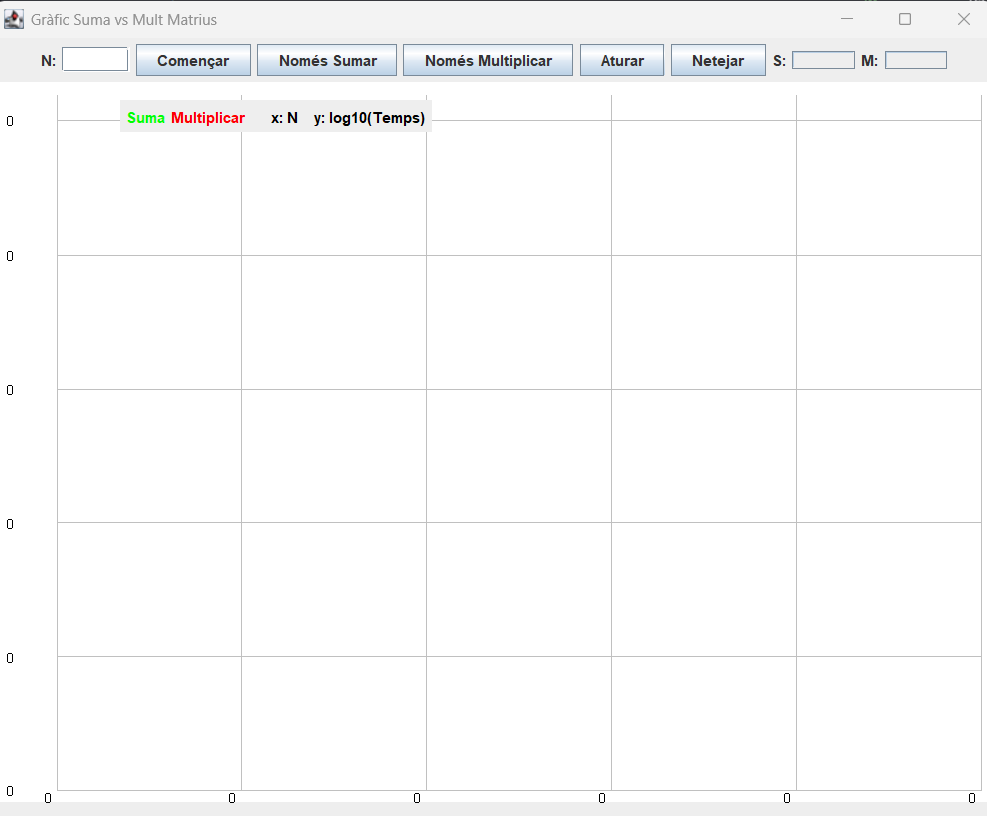
\includegraphics[width=0.4\textwidth]{png/grafica.png}}
\caption{Exemple de la interfície principal implementada.}
\label{fig:int1}
\end{figure}

    \item \textbf{Finestra de Resultats}: La finestra de resultats es crea utilitzant la classe \texttt{dibuixConstantMult} i mostra les taules amb els temps reals i esperats de les operacions de suma i producte de matrius.

\begin{figure}[htbp]
\centerline{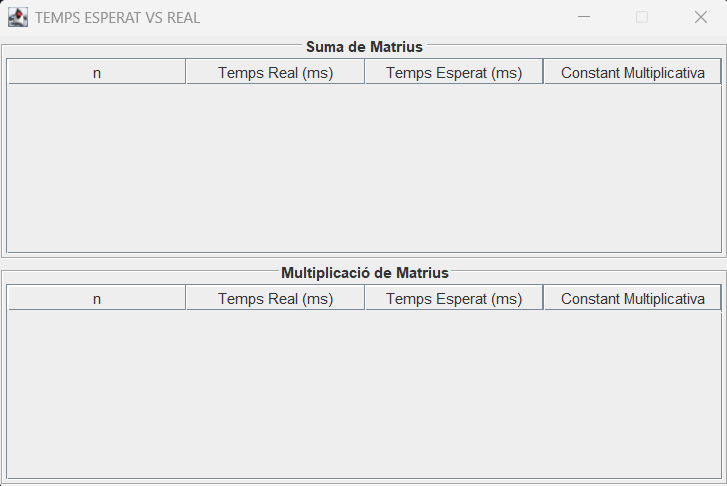
\includegraphics[width=0.4\textwidth]{png/taulaResultats.png}}
\caption{Exemple de la interfície de resultats implementada.}
\label{fig:int2}
\end{figure}

\end{itemize}

Aquestes finestres permeten a l'usuari interactuar amb l'aplicació, iniciar les operacions i visualitzar els resultats de manera clara i organitzada.


\subsection{Gestió de Fils d'Execució}
La classe \texttt{Main} utilitza un \texttt{ExecutorService} per gestionar els fils d'execució de les operacions de suma i producte de matrius. Això permet executar les operacions de manera concurrent i millorar l'eficiència de l'aplicació. Els fils es poden iniciar i aturar mitjançant missatges enviats a través de la interfície \texttt{Comunicar}.

\subsubsection{ExecutorService}
L'`ExecutorService` és una interfície que proporciona mecanismes per gestionar un conjunt de fils d'execució. En aquest projecte, s'utilitza per executar les classes \texttt{SumaM} i \texttt{MultM} en fils separats. La classe \texttt{Main} crea un `ExecutorService` amb un grup de fils fixos mitjançant el mètode \texttt{Executors.newFixedThreadPool(3)}:

\begin{lstlisting}[language=Java, basicstyle=\ttfamily\normalsize]
executorService = 
Executors.newFixedThreadPool(3);
\end{lstlisting}

Això permet tenir fins a tres fils d'execució simultanis, assegurant que les operacions de suma i producte de matrius es puguin executar de manera concurrent.

\begin{figure}[htbp]
\centerline{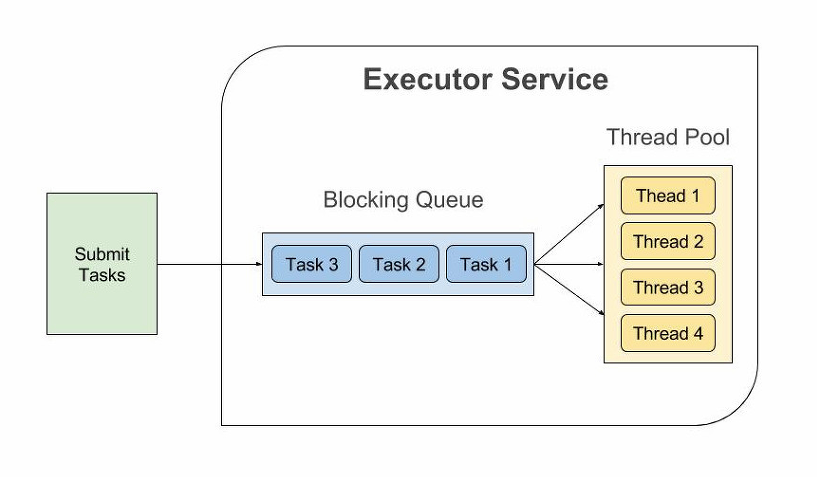
\includegraphics[width=0.45\textwidth]{png/executorService.png}}
\caption{Esquema de funcionament de l'Executor Service a Java.}
\label{fig:exeServ}
\end{figure}

\subsubsection{Inici i Aturada de Fils}
Quan l'usuari interactua amb la interfície gràfica per iniciar una operació, la classe \texttt{Main} rep un missatge mitjançant el mètode \texttt{comunicar}. Aquest mètode processa el missatge i, si és necessari, crea instàncies de les classes \texttt{SumaM} o \texttt{MultM} per executar les operacions en fils separats. Per exemple, quan es rep un missatge per iniciar les operacions de suma i producte de matrius, es creen i s'executen les instàncies de \texttt{SumaM} i \texttt{MultM}:

\begin{lstlisting}[language=Java, basicstyle=\ttfamily\normalsize]
SumaM sumaTask = new SumaM(this);
MultM multTask = new MultM(this);

procesos.add(sumaTask);
procesos.add(multTask);

executorService.execute(sumaTask);
executorService.execute(multTask);
\end{lstlisting}

Això permet que les operacions de suma i producte es puguin executar de manera concurrent, millorant l'eficiència de l'aplicació.

\subsubsection{Casos de Concurrència}
L'aplicació pot gestionar diferents casos de concurrència, depenent de les operacions que l'usuari decideixi executar:

\begin{itemize}
    \item \textbf{Execució Concurrent de Suma i Producte}: Quan l'usuari inicia les operacions de suma i producte de matrius simultàniament, les instàncies de \texttt{SumaM} i \texttt{MultM} s'executen en fils separats. Això permet que les dues operacions es realitzin al mateix temps, aprofitant els avantatges de l'execució concurrent.
    \item \textbf{Execució de Suma o Producte per Separat}: Quan l'usuari decideix executar només una de les operacions (suma o producte), només es crea i s'executa la instància corresponent (\texttt{SumaM} o \texttt{MultM}). Per exemple, si es rep un missatge per iniciar només l'operació de suma, es crida al metòde executaClass amb els següents parametres: SumM.class i n. De manera que aquest metode  crea i executa només la instància de \texttt{SumaM}:

\begin{lstlisting}[language=Java, basicstyle=\ttfamily\normalsize]
Comunicar proces = (Comunicar) classe
    .getConstructor(Main.class)
    .newInstance(this);
procesos.add(proces);
executorService.submit((Runnable) proces);
\end{lstlisting}

\end{itemize}

\subsubsection{Aturada de Fils}
Quan es rep un missatge per aturar una operació, el mètode \texttt{comunicar} de la classe \texttt{Main} envia un missatge a les instàncies de \texttt{SumaM} i \texttt{MultM} per aturar els fils d'execució. Això es fa establint la variable booleana \texttt{stop} a \texttt{true}, la qual cosa fa que el bucle principal del mètode \texttt{run} s'aturi:

\begin{lstlisting}[language=Java, basicstyle=\ttfamily\normalsize]
for (Comunicar enmarxa : procesos) {
    enmarxa.comunicar("aturar");
}
\end{lstlisting}

Això assegura que les operacions es puguin aturar de manera controlada i que els recursos es puguin alliberar correctament.

En resum, l'aplicació implementa el patró MVC i el patró per esdeveniments per gestionar les operacions de suma i producte de matrius, mostrant els resultats en una interfície gràfica desenvolupada amb Java Swing. Aquesta arquitectura permet una clara separació de responsabilitats, millorant la modularitat i mantenibilitat del codi.

\section{Resultats i Anàlisi}
S'exposen els resultats obtinguts, avaluant la modularitat del sistema i l’eficiència en la gestió d'esdeveniments. Es presenta una comparació de temps d’execució i costos computacionals.

Les següents gràfiques mostren els resultats d'executar el programa amb $N = 1000$.
\begin{figure}[htbp]
\centerline{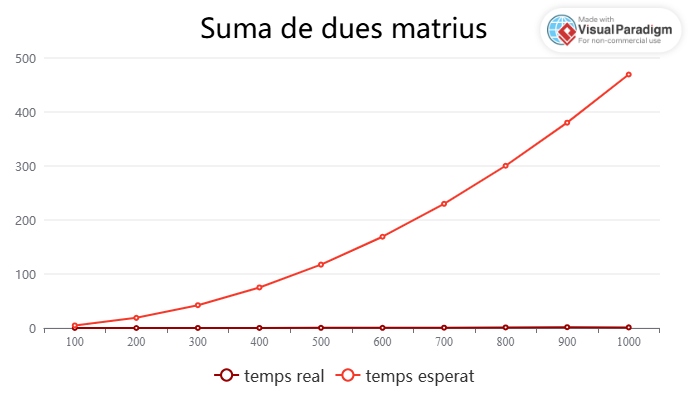
\includegraphics[width=0.4\textwidth]{png/figuera6.png}}
\caption{Gràfica amb els resultats de sumar dues matrius.}
\label{fig:int2}
\end{figure}

\begin{figure}[htbp]
\centerline{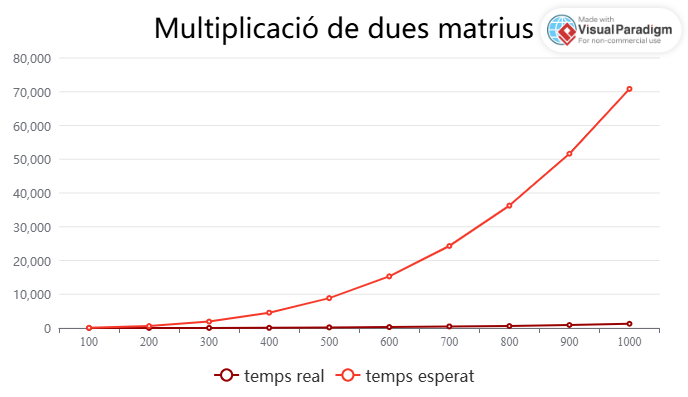
\includegraphics[width=0.4\textwidth]{png/figuera7.png}}
\caption{Gràfica amb els resultats de sumar dues matrius.}
\label{fig:int2}
\end{figure}
Com es pot veure, el temps esperat de la \textbf{Figura 6} creix de manera quadràtica, seguint una funció $n^2$. Tot i ser ràpid, aquest creixement és més lent que el de la multiplicació de matrius, que té un creixement cúbic $n^3$. Aquest darrer implica que el temps d'execució es dispara quan augmenta la mida de la matriu, fent inviable l'algorisme \texttt{multiplicar} per dimensions molt grans.

A més, hi ha una diferència clara entre el temps real i l’esperat en ambdues gràfiques. El temps esperat es determina mitjançant una constant multiplicativa calculada prèviament, que aproxima el comportament asimptòtic de l’algorisme. Aquesta discrepància existeix perquè el temps esperat marca una cota superior del temps d’execució en el pitjor cas.

Cal considerar que el càlcul està simplificat i no inclou factors com la gestió de memòria, l’eficiència de la caché o les optimitzacions del compilador, que poden influir en el temps real d’execució. Aquí només analitzem el temps pur de les operacions de suma i multiplicació de la classe \texttt{Matriu}, sense tenir en compte la càrrega inicial de dades ni altres processos interns.

En resum, el càlcul computacional és útil per estimar la durada d’un algorisme i comparar estratègies, però sempre cal validar els resultats amb proves experimentals per tenir una visió més precisa del rendiment real.

\section{Conclusions}
Es resumeixen els avantatges de l'ús del patró MVC i es proposen possibles millores futures per optimitzar el sistema.

Com s'ha mencionat prèviament i en diferents seccions de la memòria, el patró MVC permet separar millor els mòduls d'un programa, facilitant una programació més modular, escalable i fàcil de mantenir. També afavoreix la realització de proves unitàries i l’adaptació a nous requisits, ja que cada component pot evolucionar independentment.

\begin{thebibliography}{9}

\bibitem{oracleExecutorService}
Oracle. (2014). \textit{ExecutorService Interface (Java Platform SE 8)}. Recuperat de: \url{https://docs.oracle.com/javase/8/docs/api/java/util/concurrent/ExecutorService.html}

\bibitem{mvcPattern}
GeeksforGeeks. (2021). \textit{MVC Design Pattern}. Recuperat de: \url{https://www.geeksforgeeks.org/mvc-design-pattern/}

\bibitem{mvcBenefits}
GeeksforGeeks. (2021). \textit{Benefit of Using MVC}. Recuperat de: \url{https://www.geeksforgeeks.org/benefit-of-using-mvc/}

\bibitem{bigOAnalysis}
GeeksforGeeks. (2021). \textit{Analysis of Algorithms | Big-O Analysis}. Recuperat de: \url{https://www.geeksforgeeks.org/analysis-algorithms-big-o-analysis/}

\end{thebibliography}

\end{document}


